This section describes the architecture of the vision transformer model used in this thesis, which is shown Figure \ref{fig:vit}. Since sleep staging as presented
here is a ``sequence-to-one'' problem, feedback is not applicable and thus the decoder stack present in a more traditional transformer is not needed. The patch divide step and
first dense (known as ``patch projection'' in \cite{dosovitskiy2010image}) step are performed as data comes in from the \ac{eeg} \ac{adc} to reduce temporary storage usage. The 
patch divide step splits the input into 60 patches of 64 samples. The resulting nearly square matrix helps maximize utilization of the accelerator described in section \ref{sec:arch},
yielding shorter inference time and lower inference energy. The patch projection step adds a layer of learned weights to the input to allow the model to capture more complex features
from the input waveform. The projection depth is known as ``embedding depth'' or \texttt{d\_model} and is a hyperparameter of the model. The model uses an embedding depth of 64,
which was determined through hyperparameter search to yield accuracies similar to embeddeding depths of 32 or 128 (see Figure \ref{fig:emd_depth_acc}) but offers lower energy
consumption when paired with 60 patches. The model then applies a learned 1D positional embedding to the patches to allow the model to learn encoder positional infromation to the \ac{eeg}
stream. The model then applies a single encoder layer consisting of a \ac{mhsa} and \ac{mlp} layer. Figure \ref{fig:enc_layer_acc} shows that accuracy does not increase as more 
encoder layers are added, so the model uses only one encoder layer to reduce the model size. The two LayerNorm layers first normalize the inputs to a Gaussian over the second dimension,
and then scale and shift the normalized values using learnable parameters with the goal of faciliting learning and containing compute unit inputs throuh reducing covariate shift. The
\ac{mhsa} layer uses a triplet of three-dimensional weights (known as ``key'', ``query'', ``value'') to favour certain regions of the encoder input. The \ac{mhsa} layer contains the majority
of the weights in the model and is the most computationally expensive part of the model. The third dimension of the weights is known as the ``number of heads'', and the model uses 8
as it was found to yield the highest accuracy as seen in Figure \ref{fig:att_heads}. The MLP head layer is a simple parametrized sequence of dense layers. Here, a single matrix was found
to yield the highest accuracy. The final dense and softmax layer is used to map the model output to the sleep stage classes. Finally, the model takes the window average of the last
three softmax vectors to stabilize the sleep stage noise. This addition has increased the model's accuracy by 2.5\% and is a novel technique in sleep staging models. Table
\ref{tab:model_param} summarizes the hyperparameters of the model.

\begin{figure}
    \centering
    \caption{High-level transformer architecture for in-situ sleep staging}
    \includegraphics[width=0.65\textwidth]{assets/vit.png}
\end{figure}
\label{fig:vit}

\begin{figure}
    \centering
    \begin{subfigure}[b]{0.45\textwidth}
        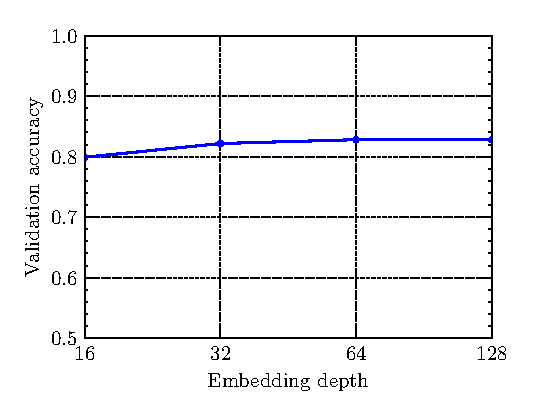
\includegraphics[width=\textwidth]{assets/acc_vs_hyperparam/emb_depth.eps}
        \caption{Accuracy vs. \texttt{d\_model}}
        \label{fig:emd_depth_acc}
    \end{subfigure}
    \hfill
    \begin{subfigure}[b]{0.45\textwidth}
        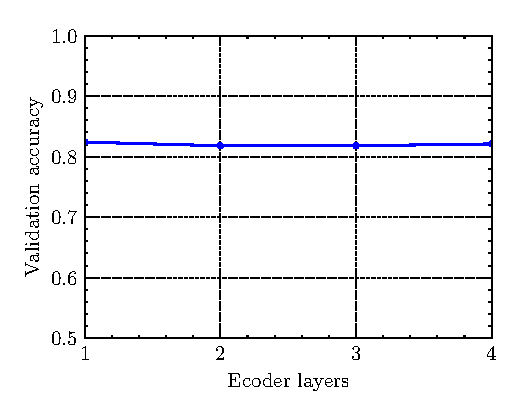
\includegraphics[width=\textwidth]{assets/acc_vs_hyperparam/enc_layer.eps}
        \caption{Accuracy vs. encoder layer count}
        \label{fig:enc_layer_acc}
    \end{subfigure}
    \vfill
    \begin{subfigure}[b]{0.45\textwidth}
        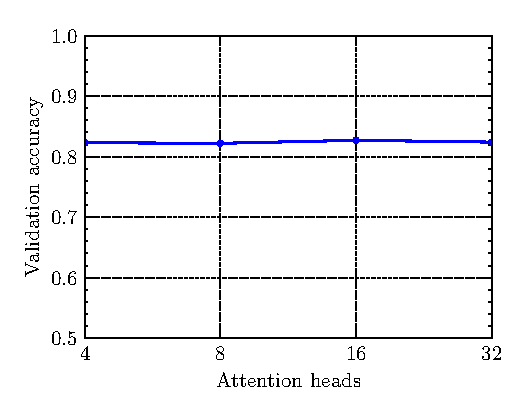
\includegraphics[width=\textwidth]{assets/acc_vs_hyperparam/att_head.eps}
        \caption{Accuracy vs. number of heads}
        \label{fig:att_heads}
    \end{subfigure}
    \hfill
    \begin{subfigure}[b]{0.45\textwidth}
        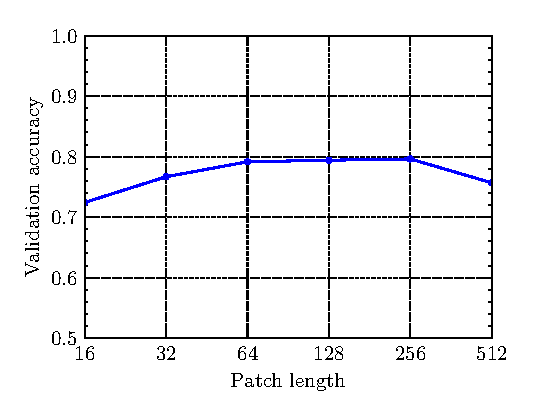
\includegraphics[width=\textwidth]{assets/acc_vs_hyperparam/patch_len.eps}
        \caption{Accuracy vs. patch length}
        \label{fig:patch_len_acc}
    \end{subfigure}
    \vfill
    \begin{subfigure}[b]{0.45\textwidth}
        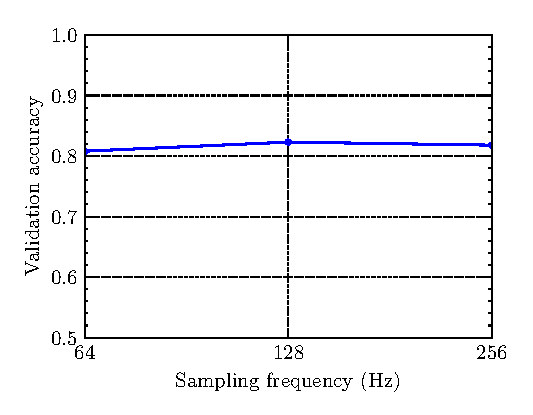
\includegraphics[width=\textwidth]{assets/acc_vs_hyperparam/sampling_freq.eps}
        \caption{Accuracy vs. sampling frequency}
        \label{fig:samp_freq_acc}
    \end{subfigure}
    \hfill
    \begin{subfigure}[b]{0.45\textwidth}
        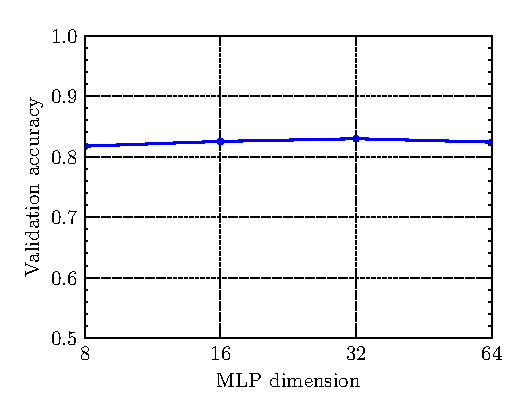
\includegraphics[width=\textwidth]{assets/acc_vs_hyperparam/mlp_dim.eps}
        \caption{Accuracy vs. MLP dimension}
        \label{fig:mlp_dense_layers_acc}
    \end{subfigure}
    \caption{Hyperparameter search results for the vision transformer model}
    \label{fig:model_hyperparameters}
\end{figure}

\begin{table}[ht]
    \centering
    \renewcommand{\arraystretch}{1.2} % Vertical spacing
    \setlength{\arrayrulewidth}{1.5pt} % Thickness of vertical lines
    \caption{Metrics and hyperparameters for vision transformer model}
    \begin{tabularx}{0.7\textwidth}{@{} *1X *1l @{}}
        \toprule
        Metric                          & Value \\\midrule
        Input channel                   & Cz-LER        \\
        Size (\# of weights)            & 31,589        \\
        Sampling frequency              & 128 Hz        \\
        Clip length                     & 30s           \\
        Patch length                    & 64 samples    \\
        Embedding depth ($d_{model}$)   & 64            \\
        \# of attention heads           & 8             \\
        \# of encoder layers            & 1             \\
        MLP dimension                   & 32            \\
        MLP head depth                  & 1             \\
        Output averaging depth          & 3 samples     \\ \bottomrule 
    \end{tabularx}
    \label{tab:model_param}
\end{table}
